\documentclass[a4paper]{article}

\usepackage{cleveref}
\usepackage{csquotes}
\usepackage{graphicx}
\usepackage{pgfplots}
\usepackage{tikz}
\usepackage[nobottomtitles]{titlesec}
\usetikzlibrary{calc}
\usetikzlibrary{datavisualization}
\usetikzlibrary{datavisualization.formats.functions}
\usetikzlibrary{math}
\usetikzlibrary{shadows}
\pgfplotsset{
	compat=newest,
	axis background/.style={
		general shadow={
			opacity=.5,
			fill=white,
			shadow scale=1.25,
		},
	},
}

\title{Signal Processing in a~BWO-Based Phase-Shift~Keying Spectrometer}
\author{}

\begin{document}

\tikzmath{
	real \lw, \F;
	\lw = 1.2;
	\F = 66;
	int \N;
	\N = 256 - 31;
	function square(\x) {
		return \x * \x;
	};
	function interference(\x) {
		return 2.5 * exp(-\x * 5.4);
	};
	function envelope(\x) {
		return 1 - exp(-\x * 10);
	};
	function line(\x, \d) {
		return exp(-\x * \lw) * cos(2*pi * \d * \x r) / (1 + square(\d / \lw));
	};
	function signal(\x, \d) {
		return (interference(\x) + line(\x, \d)) * envelope(\x);
	};
}

\tikzmath{
%	freq. diff.    A         B         C
%	0.0 * \lw:  0.09152,  2.98444, -0.00079
%	0.1 * \lw:  0.10849,  2.77384, -0.05990
%	0.2 * \lw:  0.11111,  2.40061, -0.10597
%	0.3 * \lw:  0.03690,  1.94759, -0.05741
%	0.4 * \lw: -0.02621,  2.86612,  0.01065
%	0.5 * \lw: -0.04407,  2.60926,  0.02933
%	0.6 * \lw: -0.04358,  2.47173,  0.03148
%	0.7 * \lw: -0.02683,  2.42774,  0.02270
%	0.8 * \lw: -0.01083,  2.13574,  0.01274
%	0.9 * \lw:  0.00691,  2.96903, -0.00216
%	1.0 * \lw:  0.01884,  2.69450, -0.01040
%	1.1 * \lw:  0.02834,  2.60196, -0.01683
%	1.2 * \lw:  0.03281,  2.58526, -0.02045
%	1.3 * \lw:  0.03473,  2.56706, -0.02200
%	1.4 * \lw:  0.03389,  2.56258, -0.02164
%	1.5 * \lw:  0.03157,  2.56217, -0.02022
%	1.6 * \lw:  0.02854,  2.56211, -0.01812
%	1.7 * \lw:  0.02506,  2.57265, -0.01583
%	1.8 * \lw:  0.02216,  2.57576, -0.01370
%	1.9 * \lw:  0.01944,  2.59384, -0.01190
%	2.0 * \lw:  0.01781,  2.59695, -0.01062
%	2.1 * \lw:  0.01656,  2.61406, -0.00983
%	2.2 * \lw:  0.01634,  2.61159, -0.00955
%	2.3 * \lw:  0.01641,  2.61908, -0.00964
%	2.4 * \lw:  0.01716,  2.61146, -0.01007
%	2.5 * \lw:  0.01798,  2.61083, -0.01067
%	2.6 * \lw:  0.01905,  2.60333, -0.01137
%	2.7 * \lw:  0.02000,  2.59993, -0.01204
%	2.8 * \lw:  0.02086,  2.59536, -0.01264
%	2.9 * \lw:  0.02151,  2.59210, -0.01309
%	3.0 * \lw:  0.02190,  2.59067, -0.01338
%	3.1 * \lw:  0.02208,  2.58852, -0.01350
%	3.2 * \lw:  0.02198,  2.58959, -0.01346
%	3.3 * \lw:  0.02179,  2.58866, -0.01330
%	3.4 * \lw:  0.02138,  2.59133, -0.01306
%	3.5 * \lw:  0.02100,  2.59133, -0.01277
%	3.6 * \lw:  0.02054,  2.59456, -0.01247
%	3.7 * \lw:  0.02019,  2.59493, -0.01221
%	3.8 * \lw:  0.01986,  2.59757, -0.01200
%	3.9 * \lw:  0.01969,  2.59772, -0.01187
%	4.0 * \lw:  0.01959,  2.59900, -0.01180
%	4.1 * \lw:  0.01963,  2.59865, -0.01182
%	4.2 * \lw:  0.01974,  2.59848, -0.01189
%	4.3 * \lw:  0.01991,  2.59781, -0.01201
%	4.4 * \lw:  0.02013,  2.59669, -0.01216
%	4.5 * \lw:  0.02034,  2.59611, -0.01231
%	4.6 * \lw:  0.02055,  2.59473, -0.01245
%	4.7 * \lw:  0.02070,  2.59454, -0.01256
%	4.8 * \lw:  0.02082,  2.59342, -0.01264
%	4.9 * \lw:  0.02086,  2.59372, -0.01267
%	5.0 * \lw:  0.02086,  2.59311, -0.01267
	function fit(\x, \A, \B, \C) {
		return \A * square(\x - \B) + \C;
	};
}

\maketitle

\begin{abstract}
The article covers the stages which the spectrometer application takes to process the signal acquired by a Schottky diode receiver of the spectrometer. First, we discuss what the signal consists of. Then, we uncover unpleasant nuances of the time-domain signal processing. Finally, we combine the results to build the spectrum we present.
\end{abstract}

\section{The Setup}\label{sec:The Setup}

The spectrometer consists of a BWO-based radiation source, a gas volume with walls transparent to the BWO radiation, and a receiver made up of a Schottky diode, an AC amplifier, and a DC one. The latter is used to cancel the variations of the BWO power out and is not the topic of the further article.

The gas volume is basically a pipe of a silica or metal, with transparent ends to let the radiation pass through. The gas inside is kept under low pressure to make the absorption lines narrower and more distinguishable. The BWO and the receiver reside at the opposite ends of the pipe, so that the EM wave travels all the length of the volume.

With the phase-locked loop on, the BWO produces such a narrow spectral line that we can easily neglect its width for the following discussions. Thus, we consider the BWO to be a monochromatic source. As the emission phase is locked, the BWO radiation is close to a pure sine wave, quite like what a perfect laser would produce.

\section{The Transient Signal from a Phase Change}\label{sec:The Transient Signal from a Phase Change}

\begin{figure}
	\hspace*{0.3in}
	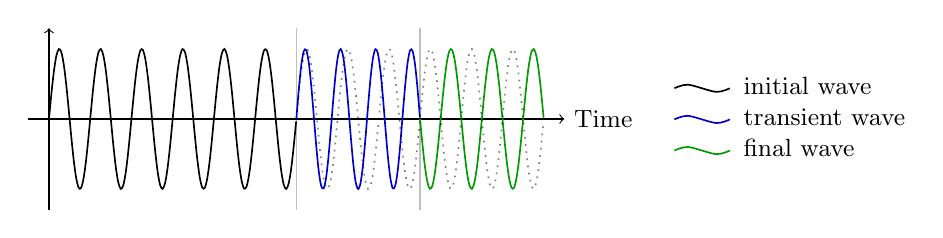
\begin{tikzpicture}[remember picture]
		\datavisualization [school book axes,
			visualize as smooth line/.list={initial,old,transient,final},
			style sheet=strong colors,
			initial={label in legend={text=initial wave}},
			transient={label in legend={text=transient wave}},
			final={label in legend={text=final wave}},
			old={style={black, opacity=0.5, dotted}},
			data/format=function,
			all axes={ticks=none},
			x axis={
				grid={
					major={
						at={
							(pi),
							(1.5 * pi),
						}
					}
				},
				ticks=none,
				label=Time,
			},
			y axis={
				ticks=none,
				length=0.7in,
			},
		]
		data [set=initial] {
			var x : interval [0:pi] step (0.01*pi);
			func y = sin(\value x r * 12);
		}
		data [set=old] {
			var x : interval [pi:2*pi] step (0.01*pi);
			func y = sin(\value x r * 12);
		}
		data [set=transient] {
			var x : interval [pi:1.5*pi] step (0.01*pi);
			func y = sin((\value x - pi) r * 14);
		}
		data [set=final] {
			var x : interval [1.5*pi:2*pi] step (0.01*pi);
			func y = -sin((\value x - 1.5*pi) r * 12);
		}
		;
	\end{tikzpicture}\\
	\hspace*{0.3in}
	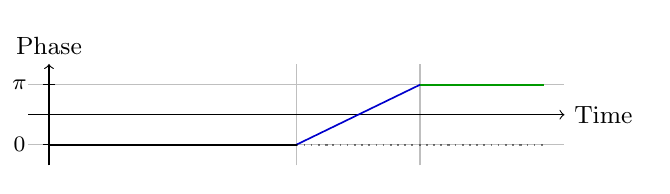
\begin{tikzpicture}[remember picture]
		\datavisualization [school book axes,
			visualize as smooth line/.list={initial,old,transient,final},
			style sheet=strong colors,
			old={style={black, opacity=0.5, dotted}},
			data/format=function,
			x axis={
				grid={
					major={
						at={
							(pi),
							(1.5 * pi),
						}
					}
				},
				ticks=none,
				label=Time,
			},
			y axis={
				ticks and grid={
					major={
						at={
							-1.0 as \makebox[0pt]{\hspace*{-1em}\hspace*{-1ex}$0$},
							 1.0 as \makebox[0pt]{\hspace*{-1em}\hspace*{-1ex}$\pi$},
						}
					}
				},
				label=\makebox[0pt]{Phase},
				length=0.3in,
			},
		]
		data [set=initial] {
			var x : interval [0:pi] samples 2;
			func y = -1;
		}
		data [set=old] {
			var x : interval [pi:2*pi] samples 2;
			func y = -1;
		}
		data [set=transient] {
			var x : interval [pi:1.5*pi] samples 2;
			func y = 4.0 * (\value x - pi) / pi - 1.0;
		}
		data [set=final] {
			var x : interval [1.5*pi:2*pi] samples 2;
			func y = 1;
		}
		;
	\end{tikzpicture}\\
	\hspace*{0.3in}
	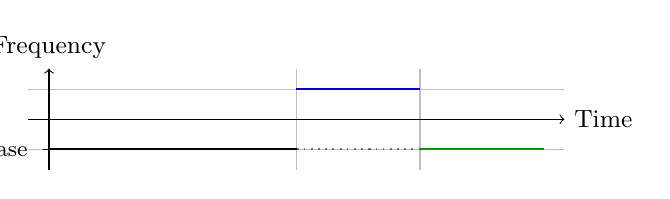
\begin{tikzpicture}[remember picture]
		\datavisualization [school book axes,
			visualize as smooth line/.list={initial,old,transient,final},
			style sheet=strong colors,
			old={style={black, opacity=0.5, dotted}},
			data/format=function,
			x axis={
				grid={
					major={
						at={
							(pi),
							(1.5 * pi),
						}
					}
				},
				ticks=none,
				label=Time,
			},
			y axis={
				grid={
					major={
						at={
							-1.0,
							1.0,
						}
					}
				},
				ticks={
					major={
						at={
							-1.0 as \makebox[0pt]{\hspace*{-1em}\hspace*{-4ex}base},
						}
					}
				},
				label=\makebox[0pt]{Frequency},
				length=0.3in,
			},
		]
		data [set=initial] {
			var x : interval [0:pi] samples 2;
			func y = -1;
		}
		data [set=old] {
			var x : interval [pi:1.5*pi] samples 2;
			func y = -1;
		}
		data [set=transient] {
			var x : interval [pi:1.5*pi] samples 2;
			func y = 1;
		}
		data [set=final] {
			var x : interval [1.5*pi:2*pi] samples 2;
			func y = -1;
		}
		;
	\end{tikzpicture}
	\caption{An illustrative plot depicting how the phase of an EM wave changes. In the upper plot, the black line and black dots are the initial wave, the green line is a wave having the opposite phase to the initial one, and the blue part is where the frequency deviates to build the phase difference up. The two other plots show how the wave phase and frequency change over time.}
	\label{fig:psk wave}
\end{figure}

The phase of the BWO radiation changes via altering the frequency of the latter (\cref{fig:psk wave}). Depending on the voltage on the output of the phase detector and a noise compound, the frequency may decrease or increase for a little while.

\begin{figure}
	\begin{tikzpicture}[remember picture]
		\datavisualization [school book axes,
		visualize as smooth line/.list={interference, relaxation, envelope, sum},
		style sheet=strong colors,
		interference={label in legend={text=interference due to the phase switch}},
		relaxation={label in legend={text=absorption line ringdown}},
		envelope={label in legend={text=AC amplifier reaction}, style={dashed}},
		sum={label in legend={text=total signal}, style={line width=2pt}},
		data/format=function,
		all axes={ticks=none},
		x axis={label=Time, length=0.3\linewidth},
		y axis={label=Voltage, length=1in},
		]
		data [set=interference] {
			var x : interval [0:255/\F] samples 255;
			func y = interference(\value x);
		}
		data [set=relaxation] {
			var x : interval [0:255/\F] samples 255;
			func y = line(\value x, 0.0);
		}
		data [set=envelope] {
			var x : interval [0:255/\F] samples 255;
			func y = envelope(\value x);
		}
		data [set=sum] {
			var x : interval [0:255/\F] samples 255;
			func y = signal(\value x, 0.0);
		}
		;
	\end{tikzpicture}
	\caption{The components of the AC signal coming from the Schottky diode.}
	\label{fig:receiver signal}
\end{figure}

As the Schottky diode is non-linear, it produces a DC voltage when being irradiated. Unless the properties of the radiation change one way or another, the voltage is fairly stable. However, when the BWO frequency differs, its power changes as well. The sensitivity of the diode varies with frequency as well. In the time domain, the two phenomena result in a bump (see the black curve in \cref{fig:receiver signal}), abruptly ending when the BWO frequency comes back.

The similar short interference might happen when the gas volume identifies itself as a resonator. In this case, the radiation doesn't leave it instantly, reflecting from the walls. Until the old wave noticeably persists, two signals come to the receiver simultaneously: the sine wave that the BWO was emitting right before we decided to change its phase, and the wave of a close frequency, which the BWO is emitting. The signals interfere, producing a sharp peak of voltage on the Schottky diode. Even if there is a way of telling this effect from what's described in the previous paragraph, there is no practical need for that.

When the BWO frequency is far from the resonant one of a gas between the BWO horn and the receiver, the interference is the only AC signal coming from the Schottky diode. However, within an absorption line, a transient process induced by the phase-shift keying adds up. In the center of the line, it's just an exponent (the red curve in \cref{fig:receiver signal}). The dependence originates from the quantum nature of the emission and absorption of light. For a gas molecule, which has not interacted with the EM wave, it doesn't matter, how long it has not done for. Regardless of the time passed, there is a constant probability of the interaction. But the longer we wait, the fewer molecules have not been influenced by the radiation. That's precisely the way radioactive decay behaves.

If the BWO frequency doesn't match the line center exactly, but differs just a little, the EM wave still interacts with the molecules. There are two reasons for that.
\begin{itemize}
	\item The gas has a temperature. This means that the molecules fly quite rapidly to experience the Doppler effect. The direction of the flight is more or less random, so there are molecules, which approach the radiation source and therefore feel more \enquote{blueish} wave, and molecules that fly away from the BWO and experience more \enquote{reddish} radiation. The speed of the movement varies, too. As there are myriads of the molecules flying, the impact of them averages into a bell-like shape of \textit{a Gaussian distribution}.
	\item The gas has a temperature. This means that the molecules fly quite rapidly and randomly collide one with another. The only outcome of the collisions is that the molecules deform for a little while and bounce back. Among the rest, the shape of a molecule determines its spectrum. During the collision, the deformation alters the shape and shifts the spectral lines. As there are myriads of the molecules flying, the impact of them averages into a bell-like shape of \textit{a Lorentz distribution}.
\end{itemize}

\begin{figure}
	\begin{tikzpicture}[remember picture]
		\datavisualization [school book axes,
		visualize as smooth line/.list={6,...,0},
		style sheet=strong colors,
		style sheet=vary thickness,
		0={label in legend={text=at the central frequency of the line}},
		1={label in legend={text=off by 1/8 of the line width}},
		2={label in legend={text=off by 2/8 of the line width}},
		3={label in legend={text=off by 3/8 of the line width}},
		4={label in legend={text=off by 4/8 of the line width}},
		5={label in legend={text=off by 5/8 of the line width}},
		6={label in legend={text=off by 6/8 of the line width}},
		data/format=function,
		all axes={ticks=none},
		x axis={label=Time, length=0.3\linewidth},
		y axis={label=Voltage, length=1in},
		]
		data {
			var set : {0,...,6};
			var x : interval [0:255/\F] samples 255;
			func y = line(\value x, \value{set} * \lw / 8);
		}
		;
	\end{tikzpicture}
	\caption{The signal from an absorption line at some frequency values close to the line center.}
	\label{fig:ringdown along the line}
\end{figure}

The molecules are tiny enough for quantum physics to govern their life. They can neither absorb nor emit EM radiation of an arbitrary frequency. They're bound to emit a wave of a predetermined one. That is, they emit a wave of the frequency that is slightly different from the one of the BWO radiation. When two sine waves of close frequency come to a Schottky diode, they interfere and produce a sine signal, exponentially decaying over time (\cref{fig:ringdown along the line}). The shape of the envelope has the origin we've discussed earlier. The frequency of the sine is the difference between the one of the two waves.

Finally, the AC signal from the Schottky diode gets amplified. The amplifier can't respond instantly, so the voltage it produces gets smoothed. The fastest change of the signal during the phase-shift keying occurs when the detector feels the rapid change of the BWO frequency. As it marks the beginning of a single interaction with the gas, we can describe it as an exponential envelope for the whole signal (see the blue and the green curves in \cref{fig:receiver signal}).

And there is always noise.

\section{The Approximation of the Transient Signal}\label{sec:The Approximation of the Transient Signal}

\begin{minipage}{\linewidth}
	\begin{center}
		\rule{0.75\linewidth}{0.2em}\\[0.5em]

		\begin{minipage}{0.75\linewidth}
			\begin{center}
				The following material may cause conflicting feelings. Reader discretion is advised.
			\end{center}
		\end{minipage}

		\rule{0.75\linewidth}{0.2em}\\[0.5em]
	\end{center}
\end{minipage}

\subsection{The Direct Approach}\label{subsec:The Direct Approach}

\begin{figure}
	\begin{tikzpicture}[remember picture]
		\datavisualization [school book axes,
		visualize as smooth line/.list={interference, signal at center, fit for signal at center, signal half line width off, fit for signal half line width off},
		interference={style={gray, solid}, label in legend={text=interference}},
		signal at center={style={black, solid}, label in legend={text=signal at the center of the line}},
		fit for signal at center={style={black, dashed}, label in legend={text=fit at the center of the line}},
		signal half line width off={style={red, solid}, label in legend={text=signal half a line width off the center}},
		fit for signal half line width off={style={red, dashed}, label in legend={text=fit half a line width off the center}},
		data/format=function,
		all axes={ticks=none},
		x axis={label=Time, length=0.3\linewidth},
		y axis={label=Voltage, length=1in},
		]
		data [set=interference] {
			var x : interval [0:255/\F] samples 255;
			func y = interference(\value x) * envelope(\value x);
		}
		data [set=signal at center] {
			var x : interval [0:255/\F] samples 255;
			func y = signal(\value x, 0.0);
		}
		data [set=fit for signal at center] {
			var x : interval [31/\F:255/\F] samples 225;
			func y = fit(\value x, 0.09152,  2.98444, -0.00079);
		}
		data [set=signal half line width off] {
			var x : interval [0:255/\F] samples 255;
			func y = signal(\value x, 0.5 * \lw);
		}
		data [set=fit for signal half line width off] {
			var x : interval [31/\F:255/\F] samples 225;
			func y = fit(\value x, -0.04407,  2.60926,  0.02933);
		}
		info {
			\draw [blue, dotted, thick] (visualization cs: x={(31/\F)}, y=-0.25) rectangle (visualization cs: x={(255/\F)}, y=0.67);
			\draw [black, dotted] (visualization cs: x={(255/\F)}, y={(fit(255/\F, 0.09152,  2.98444, -0.00079))}) -- +(visualization cs: x={(-\N/\F)}, y=0);
			\draw [black, solid, latex-latex] (visualization cs: x={(31/\F)}, y={(fit(255/\F, 0.09152,  2.98444, -0.00079))}) -- (visualization cs: x={(31/\F)}, y={(fit(31/\F, 0.09152,  2.98444, -0.00079))});
			\draw [red, dotted] (visualization cs: x={(255/\F)}, y={(fit(255/\F, -0.04407,  2.60926,  0.02933))}) -- +(visualization cs: x={(-\N/\F)}, y=0);
			\draw [red, solid, latex-latex] (visualization cs: x={(31/\F)}, y={(fit(255/\F, -0.04407,  2.60926,  0.02933))}) -- (visualization cs: x={(31/\F)}, y={(fit(31/\F, -0.04407,  2.60926,  0.02933))});
		}
		;
	\end{tikzpicture}
	\caption{The parabolic approximation of the signal from an absorption line at the line center and half a line width off the central frequency. The blue rectangle marks the range used to calculate the approximation. At the left edge of the rectangle, the black and (merely visible) red arrows depict the signal magnitude as we record it for the frequency values.}
	\label{fig:parabola fit}
\end{figure}

We try to tell the absorption by a line from the interference of the phase change. The latter decays much faster than the signal from the line. So, we reject the beginning of the time-domain record for good (see the blue rectangle in \cref{fig:parabola fit}).

It's hard to fight noise further than obtaining a single point, a scalar value. As we expect, say, an exponential signal to appear if there is an absorption line, we approximate the rest of the data with a polynomial. Namely, a parabola (see the black dashed line in \cref{fig:parabola fit}). That's fairly quick to do.

From the fit, we require just the difference between the height of the first point and the one of the last (see the black arrow in \cref{fig:parabola fit}). That's what we take as the line strength and plot against time of the BWO frequency.

The disaster strikes when the signal we obtain is far from exponential (like the red solid line in \cref{fig:parabola fit}). It takes place quite close to the center of an absorption line. There, a parabola merely fits the dependence, and the difference between the edge points of the parabola may even change its sign, despite the BWO frequency is still well within the absorption line (see the red dashed line in \cref{fig:parabola fit}).

Despite the corruption of the line shape, the seemingly inappropriate approximation presents as with a mean of telling whether a bump on a spectrum is an actual line or just an interference.

\subsection{The Slowly Changing Interference}\label{subsec:The Slowly Changing Interference}

In practice, the interference from the phase switch doesn't vary much for close frequency points. By \enquote{close}, we mean the values separated by no more than the width of an absorption line. To reduce the interference, we compare the signals at a certain frequency (let us call it the central one) with the ones at the frequency, shifted both ways by the width of the absorption line we expect to detect. Basically, we subtract the mean of the latter signals from the one at the central frequency. Although the approach does reduce the interference, it doesn't cancel it out completely, and therefore the further algorithm stays the same as in \Cref{subsec:The Direct Approach}.

\clearpage

\section{The Absorption Line}\label{sec:The Absorption Line}

\begin{figure}[h!]
	\begin{tikzpicture}[remember picture]
		\datavisualization [school book axes,
			visualize as smooth line/.list={Lorentz, approximation},
			legend=below,
			style sheet=strong colors,
			Lorentz={label in legend={text=Lorentz shape}},
			approximation={label in legend={text=approximation result}},
			data/format=function,
			x axis={
				ticks and grid={
					major={
						at={
							(-4.0 * \lw) as $-4.0$,
							(-3.0 * \lw) as $-3.0$,
							(-2.0 * \lw) as $-2.0$,
							(-1.5 * \lw) as $-1.5$,
							(-\lw) as $-1.0$,
							(-0.5 * \lw) as $-0.5$,
							0,
							(0.5 * \lw) as $0.5$,
							(\lw) as $1.0$,
							(1.5 * \lw) as $1.5$,
							(2.0 * \lw) as $2.0$,
							(3.0 * \lw) as $3.0$,
							(4.0 * \lw) as $4.0$,
						}
					}
				},
				ticks={stack'=1.0em},
				label={\hspace*{-0.7in}\raisebox{1em}{Frequency}},
				length={\linewidth-0.25in},
			},
			y axis={
				ticks and grid={
					major={
						at={
							1.0,
							0.5,
						}
					}
				},
				label=Signal,
				length=\linewidth,
			},
		]
		data [set=Lorentz] {
			var x : interval [-5*\lw:5*\lw] samples 255;
			func y = 1 / (1 + square(\value x / \lw));
		}
		data [format=named, set=approximation] {
%			var t : interval [31/\F:255/\F] samples 225;
%			p = polyfit(t, signal(t, x), 2)
%			a = p[0]
%			b = -p[1] / (2. * p[0])
%			c = p[2] - p[1]**2 / (4. * p[0])
%			y= fit(31/66, a, b, c) - fit(255/66, a, b, c)
			x=(-5.0 * \lw), y=0.06039024404973334
			x=(-4.9 * \lw), y=0.0604589008430699
			x=(-4.8 * \lw), y=0.0603204983725208
			x=(-4.7 * \lw), y=0.06011788642154373
			x=(-4.6 * \lw), y=0.059717983413288905
			x=(-4.5 * \lw), y=0.059287633377423266
			x=(-4.4 * \lw), y=0.05875499538493379
			x=(-4.3 * \lw), y=0.05827043552310482
			x=(-4.2 * \lw), y=0.05784501891750558
			x=(-4.1 * \lw), y=0.0575559538447706
			x=(-4.0 * \lw), y=0.05750137800886406
			x=(-3.9 * \lw), y=0.05762577301729203
			x=(-3.8 * \lw), y=0.05810251640007618
			x=(-3.7 * \lw), y=0.05870156989068175
			x=(-3.6 * \lw), y=0.05964989786752393
			x=(-3.5 * \lw), y=0.06054192942236135
			x=(-3.4 * \lw), y=0.06163392355407378
			x=(-3.3 * \lw), y=0.06240243858716785
			x=(-3.2 * \lw), y=0.06310952790426783
			x=(-3.1 * \lw), y=0.06323514604954142
			x=(-3.0 * \lw), y=0.06302040779163362
			x=(-2.9 * \lw), y=0.06211978777557987
			x=(-2.8 * \lw), y=0.06071153272090712
			x=(-2.7 * \lw), y=0.05881178917504334
			x=(-2.6 * \lw), y=0.05646303621992728
			x=(-2.5 * \lw), y=0.05419623778253944
			x=(-2.4 * \lw), y=0.05180333673988275
			x=(-2.3 * \lw), y=0.05039143586230188
			x=(-2.2 * \lw), y=0.04935086507577116
			x=(-2.1 * \lw), y=0.0502794522268092
			x=(-2.0 * \lw), y=0.05201231127332384
			x=(-1.9 * \lw), y=0.056363911710837114
			x=(-1.8 * \lw), y=0.061529439183702274
			x=(-1.7 * \lw), y=0.06905604645041744
			x=(-1.6 * \lw), y=0.07659891984155118
			x=(-1.5 * \lw), y=0.08475133373896204
			x=(-1.4 * \lw), y=0.09108157313592705
			x=(-1.3 * \lw), y=0.09439395480653535
			x=(-1.2 * \lw), y=0.09322032445969491
			x=(-1.1 * \lw), y=0.0837469995730622
			x=(-1.0 * \lw), y=0.06749897829637705
			x=(-0.9 * \lw), y=0.037610081210240544
			x=(-0.8 * \lw), y=0.0022740563918155175
			x=(-0.7 * \lw), y=-0.04754365287854277
			x=(-0.6 * \lw), y=-0.0902479804334782
			x=(-0.5 * \lw), y=-0.13239973273145123
			x=(-0.4 * \lw), y=-0.12446100233526292
			x=(-0.3 * \lw), y=-0.05487570911005679
			x=(-0.2 * \lw), y=0.17643926954468866
			x=(-0.1 * \lw), y=0.44714182922162926
			x=(0.0 * \lw), y=0.5080422227088788
			x=(0.1 * \lw), y=0.4471418292216866
			x=(0.2 * \lw), y=0.1764392695448016
			x=(0.3 * \lw), y=-0.05487570911001223
			x=(0.4 * \lw), y=-0.12446100233524929
			x=(0.5 * \lw), y=-0.1323997327314606
			x=(0.6 * \lw), y=-0.09024798043349375
			x=(0.7 * \lw), y=-0.04754365287856001
			x=(0.8 * \lw), y=0.0022740563917999085
			x=(0.9 * \lw), y=0.037610081210229414
			x=(1.0 * \lw), y=0.0674989782963682
			x=(1.1 * \lw), y=0.08374699957305826
			x=(1.2 * \lw), y=0.09322032445969283
			x=(1.3 * \lw), y=0.09439395480653633
			x=(1.4 * \lw), y=0.0910815731359284
			x=(1.5 * \lw), y=0.08475133373896512
			x=(1.6 * \lw), y=0.0765989198415536
			x=(1.7 * \lw), y=0.06905604645042054
			x=(1.8 * \lw), y=0.06152943918370457
			x=(1.9 * \lw), y=0.056363911710839
			x=(2.0 * \lw), y=0.052012311273324945
			x=(2.1 * \lw), y=0.05027945222680985
			x=(2.2 * \lw), y=0.04935086507577123
			x=(2.3 * \lw), y=0.0503914358623012
			x=(2.4 * \lw), y=0.051803336739882216
			x=(2.5 * \lw), y=0.05419623778253853
			x=(2.6 * \lw), y=0.05646303621992649
			x=(2.7 * \lw), y=0.05881178917504249
			x=(2.8 * \lw), y=0.060711532720906645
			x=(2.9 * \lw), y=0.06211978777557923
			x=(3.0 * \lw), y=0.06302040779163355
			x=(3.1 * \lw), y=0.06323514604954135
			x=(3.2 * \lw), y=0.06310952790426785
			x=(3.3 * \lw), y=0.06240243858716824
			x=(3.4 * \lw), y=0.06163392355407431
			x=(3.5 * \lw), y=0.06054192942236178
			x=(3.6 * \lw), y=0.05964989786752414
			x=(3.7 * \lw), y=0.058701569890681995
			x=(3.8 * \lw), y=0.058102516400076465
			x=(3.9 * \lw), y=0.05762577301729214
			x=(4.0 * \lw), y=0.05750137800886396
			x=(4.1 * \lw), y=0.057555953844770434
			x=(4.2 * \lw), y=0.05784501891750562
			x=(4.3 * \lw), y=0.058270435523104555
			x=(4.4 * \lw), y=0.05875499538493364
			x=(4.5 * \lw), y=0.05928763337742307
			x=(4.6 * \lw), y=0.05971798341328856
			x=(4.7 * \lw), y=0.060117886421543726
			x=(4.8 * \lw), y=0.06032049837252066
			x=(4.9 * \lw), y=0.06045890084306971
			x=(5.0 * \lw), y=0.0603902440497334
		}
		info {
			\coordinate (00) at (visualization cs: x=0.0, y=0.51);
			\coordinate (at 00) at (visualization cs: x={(0.1 * \lw)}, y=0.54);
			\draw[latex-, blue, thick] (00) -- (at 00);
			\begin{axis}[ticks=none, axis x line=bottom, axis y line=left, at={(at 00)}, width=0pt, anchor={outer south west}, footnotesize, axis line style={gray}, scale=0.3]
				\addplot[blue, domain=0:(255/66), samples=256] {signal(x, 0)};
			\end{axis}
			\coordinate (03) at (visualization cs: x={(0.3 * \lw)}, y=0.0);
			\coordinate (at 03) at (visualization cs: x={(0.5 * \lw)}, y=0.12);
			\draw[latex-, blue, thick] (03) -- (at 03);
			\begin{axis}[ticks=none, axis x line=bottom, axis y line=left, at={(at 03)}, width=0pt, anchor={outer south west}, footnotesize, axis line style={gray}, scale=0.3]
				\addplot[blue, domain=0:(255/66), samples=256] {signal(x, 0.3 * \lw)};
			\end{axis}
			\coordinate (05) at (visualization cs: x={(0.5 * \lw)}, y=-0.13);
			\coordinate (at 05) at (visualization cs: x={(0.9 * \lw)}, y=-0.13);
			\draw[latex-, blue, thick] (05) -- (at 05);
			\begin{axis}[ticks=none, axis x line=bottom, axis y line=left, at={(at 05)}, width=0pt, anchor={outer west}, footnotesize, axis line style={gray}, scale=0.3]
				\addplot[blue, domain=0:(255/66), samples=256] {signal(x, 0.5 * \lw)};
			\end{axis}
			\coordinate (30) at (visualization cs: x={(3.0 * \lw)}, y=0.063);
			\coordinate (at 30) at (visualization cs: x={(3.7 * \lw)}, y=0.11);
			\draw[latex-, blue, thick] (30) -- (at 30);
			\begin{axis}[ticks=none, axis x line=bottom, axis y line=left, at={(at 30)}, width=0pt, anchor={outer south west}, footnotesize, axis line style={gray}, scale=0.3]
				\addplot[blue, domain=0:(255/66), samples=256] {signal(x, 3.0 * \lw)};
			\end{axis}
		};
	\end{tikzpicture}
	\caption{An absorption line around its central frequency. The horizontal axis is marked in the units of the line width. The vertical axis is normalized so that the Lorentz reaches exactly 1 at its peak. The insets depict the time-domain signal obtained at the corresponding frequency.}
	\label{fig:line shape comparison}
\end{figure}

\end{document}
